% !TEX root =  ../main.tex 

\section{Personalized schedules for patients in PRIAS}
\label{sec : pers_schedule_PRIAS}

To demonstrate how the personalized schedules described in section \ref{subsec : pers_sched_approaches} work, we apply them to the patients in the PRIAS dataset. To this end, we divided the PRIAS data set into training(5938 subjects) and demonstration data sets (5 subjects). We fitted a joint model to the training data set and then used it to create a personalized schedule for subjects in demonstration data set. We fit the joint model using the R package JMbayes \citep{rizopoulosJMbayes}, which uses the Bayesian methodology to estimate the model parameters. 

\subsection{Fitting the joint model to PRIAS dataset}
The training data set contains information about 5938 prostate cancer patients who satisfied the conditions for enrollment in AS. For every patient the age at the time of induction in AS was recorded. PSA was measured every 3 months for first 2 years and every 6 months thereafter. To detect Gleason reclassification, biopsies were conducted at different time points on the basis of a predetermined schedule as well as PSA-DT as described in section \ref{sec : introduction}. For the longitudinal analysis of PSA measurements we used $\log_2 PSA$ measurements instead of the raw data. The log transformation was done because the PSA scores took very large values at the onset of disease progression. This indicated that the underlying distribution for PSA scores was right skewed. The longitudinal sub-models of the joint model we fitted is given by:

\begin{align*}
\log_2 PSA(t) &= m_i(t) + \varepsilon_i(t), \\
m_i(t) &= (\beta_0 + b_{i0}) + \beta_1 (Age-70) + \beta_2 (Age-70)^2\\ 
&+ \sum_{k=1}^4 \beta_{k+2} B_k(t,\mathcal{K}) + b_{i1} B_7(t, 0.5) + b_{i2} B_8(t, 0.5) \\
\varepsilon_i(t) & \sim N(0, \sigma^2),\\
\boldsymbol{b}_i & \sim N(0, \boldsymbol{D})
\end{align*}

The evolution of PSA levels over time is modeled flexibly using B-splines. For the fixed effects part the spline consists of 3 internal knots. The internal knots are at $\mathcal{K} =\{0.5, 1.2, 2.5\}$ years, and boundary knots are at 0 and 7 years. For the random effects part there is only 1 internal knot at 0.5 years and the boundary knots are at 0 and 7 years. The choice of knots was based on exploratory analysis as well as on the basis of model selection criteria AIC and BIC. The variable Age was median centered so avoid numerical instabilities while estimating the parameters in the model. For the survival sub-model the hazard function we fitted is given by:

\begin{equation*}
h_i(t) = h_0(t) e^{\gamma_1 (Age-70)  + \gamma_2 (Age-70)^2  \alpha_1 m_i(t) + \alpha_2 m'_i(t)}
\end{equation*}
where, $\alpha_1$ and $\alpha_2$ are measures of strength of association between hazard of Gleason reclassification and PSA value and PSA velocity, respectively. $h_0(t)$ is the baseline hazard at time t, and is modeled flexibly using P-splines\citep{eilers1996flexible}. Lastly, to fit the joint model we use the R package JMbayes \cite{rizopoulosJMbayes}, which uses a Bayesian approach for parameter estimation. The parameter estimates for the survival sub-model were estimated using Bayesian ridge methodology \citep{andrinopoulou2016bayesian}.

\subsubsection{Parameter Estimates}
The parameter estimates for the joint model we fitted to the PRIAS data set are shown in Table \ref{tab : PSA_long} and Table \ref{tab : PSA_survival}. Since the longitudinal evolution of $\log_2 PSA$ is modeled with non-linear terms, the interpretation of the coefficients corresponding to time is not straightforward. In lieu of the interpretation we present the fitted evolution of PSA over a period of 10 years for a patient who is 70 years old in Figure \ref{fig : fitted_trend_psa}. It can be seen that the after the first 6 months the PSA levels steadily increase over the follow up period. Since the model for PSA has only additive terms, this evolution remains same for all patients. The effect of Age only affects the baseline PSA score. However it is so small that it can be ignored for all practical purposes.\\

\begin{figure}[!htb]
	\centering
    \captionsetup{justification=centering}
	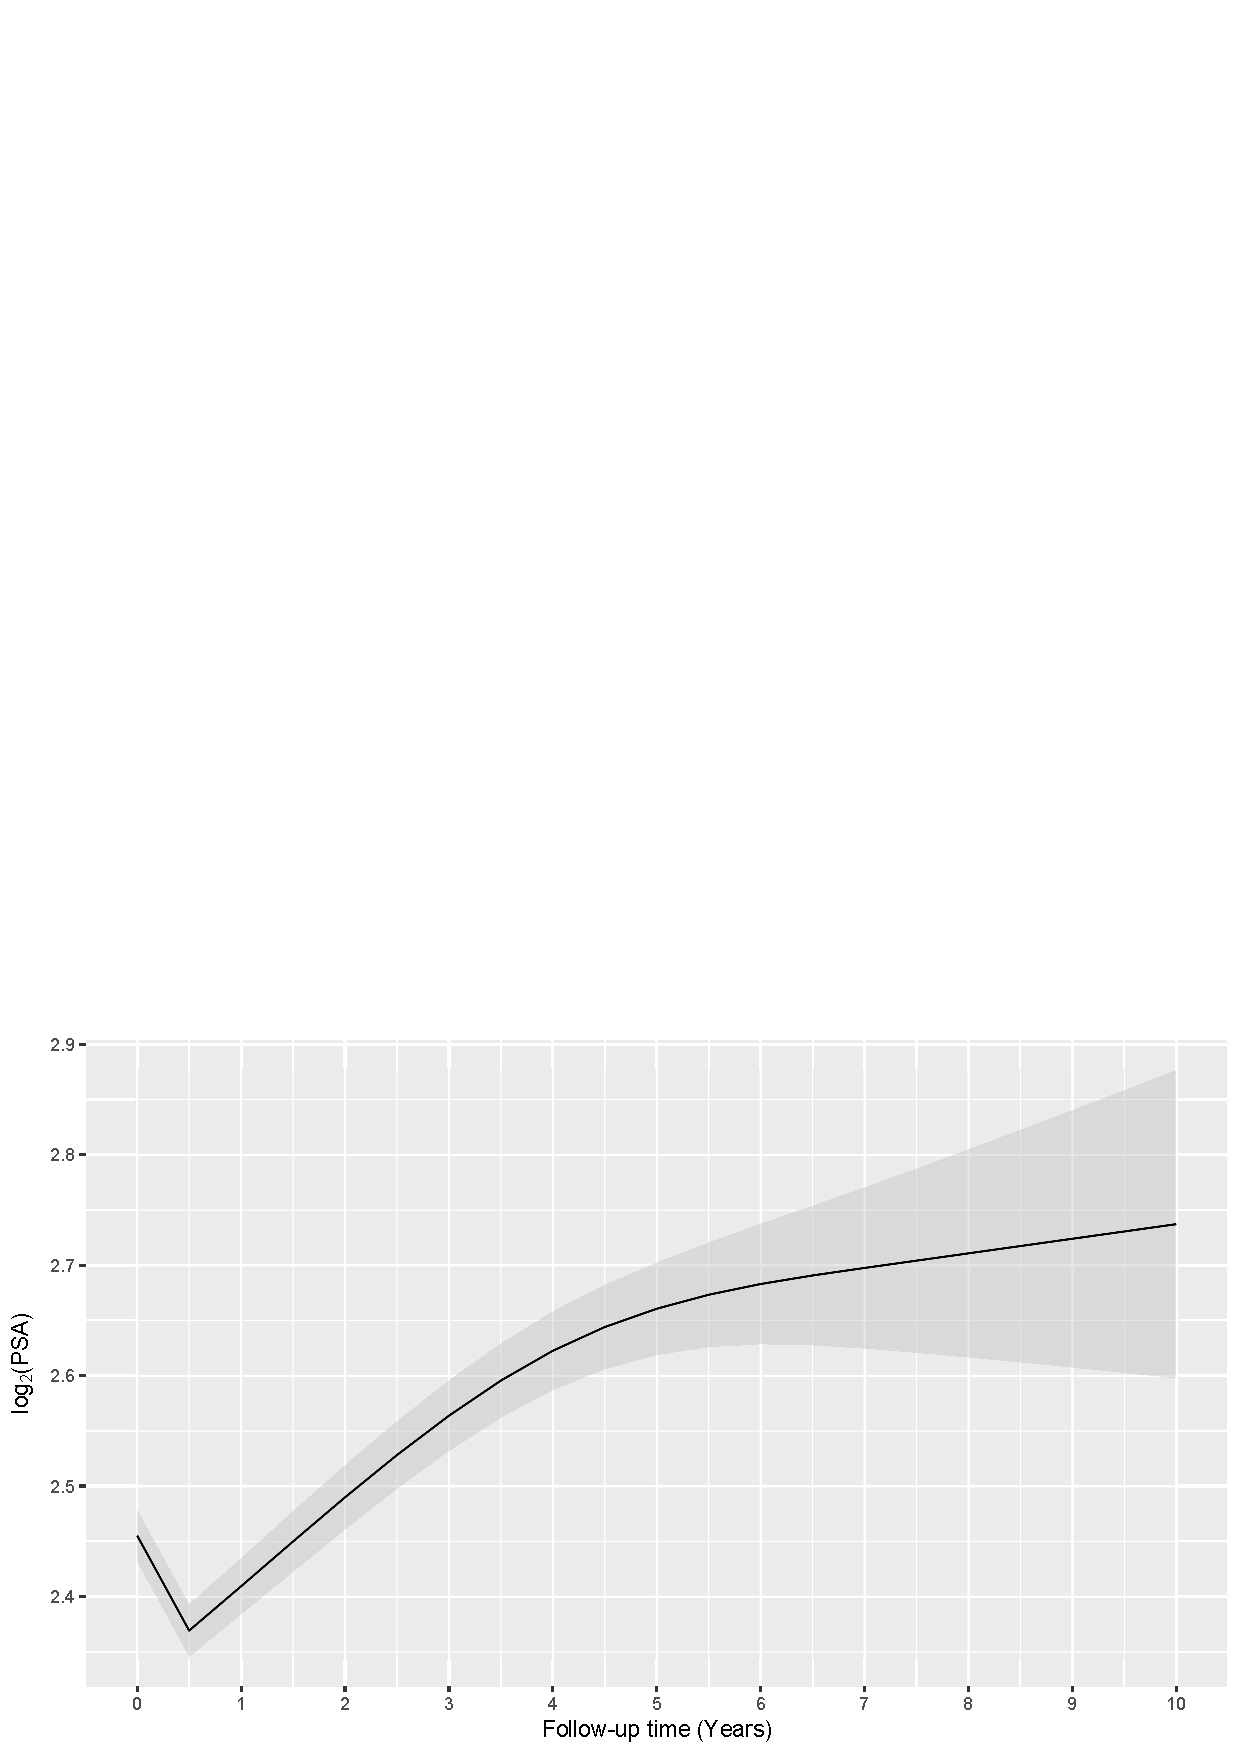
\includegraphics[width=0.8\textwidth]{fitted_trend_psa.png}
	\caption{Fitted evolution of $\log_2 PSA$ over a period of 10 years, for a patient who was inducted in AS at the Age of 70 years.}
	\label{fig : fitted_trend_psa}
\end{figure}

\begin{table}[!htb]
\centering
\caption{Longitudinal sub-model estimates for joint model.}
\label{tab : PSA_long}
\captionsetup{justification=centering}
\begin{tabular}{@{}lrrrrr@{}}
\toprule
                                     & Mean   & Std. Dev           & 2.5\%               & 97.5\%              & P              \\ \midrule
Intercept                            & 2.717  & 0.008              & 2.701               & 2.733               & \textless0.000 \\
(Age - 70)                           & 0.003  & 0.001              & 0.001               & 0.005               & 0.002          \\
(Age - 70) $\times$ (Age - 70)       & -0.001 & 1 $\times 10^{-4}$ & -7 $\times 10^{-4}$ & -4 $\times 10^{-4}$ & \textless0.000 \\
Spline: visitTimeYears{[}0, 0.5{]}   & 0.026  & 0.008              & 0.012               & 0.042               & \textless0.000 \\
Spline: visitTimeYears{[}0.5, 1.2{]} & 0.208  & 0.013              & 0.184               & 0.233               & \textless0.000 \\
Spline: visitTimeYears{[}1.2, 2.5{]} & 0.175  & 0.019              & 0.137               & 0.210               & \textless0.000 \\
Spline: visitTimeYears{[}2.5, 7{]}   & 0.309  & 0.028              & 0.256               & 0.366               & \textless0.000 \\
$\sigma$                               & 0.273  & 0.001              & 0.271               & 0.275               & \textless0.000 \\ \bottomrule
\end{tabular}
\end{table}

For the survival sub-model, the parameter estimates in Table \ref{tab : PSA_survival} show that both the $\log_2 PSA$ value and $\log_2 PSA$ velocity are associated with time to Gleason reclassification. The effect is quite strong and if at any given time point the PSA becomes approximately 4 times of its value then the hazard of Gleason reclassification  becomes 1.5 times of the original. This is valid under the condition that the $\log_2 PSA$ velocity remains the same. The effect of $\log_2 PSA$ velocity is far stronger, but it is not interpretable easily. The estimated values of the association parameters reinforces the idea that PSA measurements are indicative of Gleason reclassification. Lastly, for the effect of Age on hazard we can say that it can be safely ignored for all practical purposes.

\begin{table}[!htb]
\centering
\caption{Survival sub-model estimates for joint model.}
\captionsetup{justification=centering}
\label{tab : PSA_survival}
\begin{tabular}{@{}lrrrrr@{}}
\toprule
Variable                      & Mean   & Std. Dev & 2.5\%  & 97.5\%                 & P              \\ \midrule
Age - 70                      & 0.036  & 0.007    & 0.023  & 0.050                  & \textless0.000 \\
(Age - 70) $\times$ (Age - 70) & -0.002 & 0.001    & -0.004 & 2 $\times 10^{-4}$ & 0.016          \\
$\log_2 PSA$                  & 0.184  & 0.093    & 0.016 & 0.369                  & 0.032          \\
Slope: $\log_2 PSA$           & 1.937  & 0.278    & 1.420  & 2.525                  & \textless0.000 \\ \bottomrule
\end{tabular}
\end{table}

\subsection{Demonstration of personalized schedules}
The personalized schedules we propose in this work depend on this dynamic distribution for time to Gleason reclassification (Eq. \ref{eq : dyn_dist_fail_time}). As more PSA measurements are taken and repeat biopsies are performed, the distribution changes updated accordingly. In this section, we demonstrate the personalized schedules based on this distribution for a set of demo patients.\\

%\begin{figure}[!htb]
%	\centering
%    \captionsetup{justification=centering}
%	\includegraphics[width=0.8\textwidth]{dyn_surv_prob_2362.png}
%	\caption{Dynamic survival probability for patient with ID 2362 in the PRIAS data set.}
%	\label{fig : dyn_surv_prob_2362}
%\end{figure}

%As a first example we present the dynamic survival probability of patient 2362 from the PRIAS %data set. Patient 2362 had his last repeat biopsy at 3.78 years at which the Gleason %reclassification did not happen. The patient was later censored at 5.12 years. Using all this %information up to 5.12 years, the dynamic survival probability at any time point $u > 3.78$ %for this patient is given by the formula $Pr(T^*_{2362} \geq u| T^*_{2362} > 3.78, %\mathcal{Y}_{2362}(5.12), D_n; \theta)$. Figure \ref{fig : dyn_surv_prob_2362} shows the %dynamic survival probability for patient 2362 at time points between 5.12 and 8.12 years.

\begin{figure}[!htb]
\centering
\captionsetup{justification=centering}
\includegraphics[width=\textwidth]{prias_demo_pid_3174.png}
\caption{\label{fig : prias_demo_pid_3174} Proposed biopsy times for patient 3174 from PRIAS.}
\end{figure}

\begin{figure}[!htb]
\centering
\captionsetup{justification=centering}
\includegraphics[width=\textwidth]{prias_demo_pid_911.png}
\caption{\label{fig : prias_demo_pid_911} Proposed biopsy times for patient 3174 from PRIAS.}
\end{figure}

\begin{figure}[!htb]
\centering
\captionsetup{justification=centering}
\includegraphics[width=\textwidth]{prias_demo_pid_2340.png}
\caption{\label{fig : prias_demo_pid_2340} Proposed biopsy times for patient 3174 from PRIAS.}
\end{figure}

It can be seen in Figure \ref{fig : prias_demo_pid_3174} that the patient 3174 had a biopsy at the time of induction and none after that. The PSA for the patient increases rapidly after the 2nd year. In response to this rapid increase, the proposed biopsy times based on conditional expected failure time also decrease accordingly from 11 years to around 3.4 years. The change for risk based methods is not so drastic though. Further it can be seen that at the last visit for PSA, the proposed biopsy time is earlier than the last 5 PSA visits and similar is the case for the proposed biopsy time based on dynamic risk of failure. This is due to the fact that the last time of biopsy was time 0 (induction time) and thus the time to Gleason reclassification can take any value larger than 0. We discuss this issue in detail in section \ref{subsec : simulation_setup}.\\

Figure \ref{fig : prias_demo_pid_911} shows the PSA evolution and biopsy times for subject 911. It can be seen that this patient had 3 biopsies where Gleason reclassification did not happen. At year 2 when the patient's PSA increases rapidly the proposed failure times also decrease, whereas they increase over the next 1 year because the PSA also drops down in that time period. The fact that PSA velocity affects the biopsy times the most is also evident in the case of subject 2340, whose evolution is shown in Figure \ref{fig : prias_demo_pid_2340}. Here the rate of change at each time point is not high, and even though the PSA value reaches as high as 25 it has no effect on proposed biopsy times. This is in accordance with the estimated strength of association between PSA velocity/value and hazard of time to Gleason reclassification.\\

An interesting observation we made while creating these schedules was that the variance of time to Gleason reclassification (Eq. \ref{eq : varFailureTime}) was quite high, which essentially rules out the usefulness of conditional expected time to Gleason reclassification. Given the large difference in proposed biopsy times based on the former and methods based on dynamic risk of Gleason reclassification, one might conclude that the latter are more useful. However as we will see in the simulation study (Section \ref{sec: simulation_study}) ahead, the usefulness of the two categories of methods depends on the distribution of time to Gleason reclassification.
